\documentclass[12pt,a4paper]{scrartcl}
\usepackage[utf8]{inputenc}
\usepackage[english,russian]{babel}
\usepackage{misccorr}
\usepackage{graphicx}
\usepackage{amsmath}
\usepackage{amsfonts}
\usepackage{verbatim}
\usepackage{listings}
\usepackage{pgfplots}
\usepackage{graphicx}
\usepackage{pdfpages}
\usepackage{multirow}

\DeclareUnicodeCharacter{03BC}{\ensuremath{\mu}}
\DeclareUnicodeCharacter{03B3}{\ensuremath{\gamma}}
\DeclareUnicodeCharacter{03C3}{\ensuremath{\sigma}}
\DeclareUnicodeCharacter{03B8}{\ensuremath{\theta}}
\DeclareUnicodeCharacter{03C7}{\ensuremath{\chi}}
\DeclareUnicodeCharacter{03B1}{\ensuremath{\alpha}}

\usepackage{algorithm}
\usepackage{algpseudocode}




% Настройки листингов.
\lstset{tabsize=4,
	breaklines,
	columns=fullflexible,
	flexiblecolumns,
	numbers=left,
	numberstyle={\footnotesize},
	extendedchars=\true
}
\lstdefinelanguage{MyP}{
	language=Python,
	ndkeywordstyle=\color{darkgray}\bfseries,
	identifierstyle=\color{black},
	morecomment=[n]{/**}{*/},
	commentstyle=\color{blue}\ttfamily,
	stringstyle=\color{red}\ttfamily,
	morestring=[b]",
	showstringspaces=false,
	morecomment=[l][\color{gray}]{//},
	keepspaces=true,
	escapechar=\%,
	texcl=true
}

\begin{document}
%\begin{titlepage}
%\newpage
%\begin{figure}[H]
%	\centering
%	
\includegraphics[width=1\linewidth]{head}
%\end{figure}

\vspace{5cm}
\begin{center}
\Large Отчёт по лабораторной работе №1 \\ По дисциплине «Математическое моделирование» \\ Тема: «Приближенный аналитический метод Пикара в сравнении с численными методами» 
\end{center}

\vspace{6em}
\begin{flushright}
Студент: \hrulefill Барсуков Н.М. \\
\vspace{1.5em}
Группа: \hrulefill ИУ7-66Б\\
\vspace{1.5em}
Преподаватель: \hrulefill Градов В.М\\
\vspace{1.5em}
\end{flushright}
\vspace{\fill}
\begin{center}
Москва, 2020
\end{center}
%\end{titlepage}

\newpage
\tableofcontents

\newpage
\section{Введение}
	Класс дифференциальных уравнение, которые интегрируются в явном виде очень мал и найти общее решение в квадратурах удается лишь для узкого класса функций. 
	В связи с этим возникает потребность в приближенных методах интегрирования.
	
\section {Аналитическая часть} 

	\textbf{Целью работы} является получение навыков решения задачи Коши для ОДУ методами Пикара и явными и неявными методами Эйлера.
	
	\textbf{Исходные данные:}
	\begin{enumerate}
		\item ОДУ, не имеющее аналитического решения: \newline$u`(x) = u^2 + x^2$; \newline$u(0) = 0$
	\end{enumerate}
	
	
	Для выполнения поставленной цели необходимо выполнить следующие задачи:
	\begin{enumerate}
		\item Поставить задачу Коши для ОДУ
		\item Понять какие методы существуют
		\item Рассмотреть конкретные методы для решения поставленной задачи Коши: \begin{enumerate}
			\item Метод Пикара (Приближения 1 - 4)
			\item Метод ломанных (Явный)
			\item Метод Рунге-Кутта 2 порядка
			\item Метод Рунге-Кутта 4 порядка
		\end{enumerate}
	\end{enumerate}

	\subsection{Задача Коши}
	Задача Коши - одна из основных задачи теории дифференциальных уравнений (обыкновенных и с частными производными); состоит в нохождении решения (интеграла) дифференциального уравнения, удовлетворяющего так называемым начальным условиям
	
	\subsection{Методы}
	
	Методы решения ДУ можно разбить на точные, приближенные и численные. 
	
	К точным относятся методы, позволяющие выразить решение дифференциального уравнения, через элементарные функции. 
	Либо представить его в при помощи квадратур от элементарных функций. Однако классы, для которых разработаны методы получения точных решенений, сравнительно узки и охватывают только малую часть возникающих на практике задач. \textbf{В данной лабораторной работе рассматриваться не будут }
	
	Приближенными будем называть методы, в которых решение получается как предел $u(x)$ некоторой последовательности $y_n(x)$, причем $y_n(x)$ выражается через элементарные функции или при помощи квадратур. 
	Ограничиваясь конечным числом n, получаем приближенное выражение для $u(x)$. 
	Эти методы удобны лишь в том случае, когда большую часть промежуточных выкладок удается сделать точно. Примером может служить метод Пикара.
	Это выполнимо лишь для сравнительно простых задач, что сильно сужает область применения приближенных методов.
	
	Численные методы - это алгоритмы вычисления приближенных (а иногда - точных) значений искомого решения $u(x)$ на некоторой выбранной сетке значений аргумента $x_n$. Численные методы не позволяют найти общего решения системы; они могут дать только какое-то частное решение. Зато данные методы применимы к очень широким классам уравнений и всем типам задач для них.
	
	Рассмотрим детально представителей данных методологий
	
	\subsubsection{Метод Пикара}
	
	Метод Пикара - это приближенный метод решения, являющийся обобщением метода последовательных приближений.
	
	\begin{align*}
	\end{align*}
	
	Рассмотрим пример из лекций:
	\begin{align*}
		\big \{ 
			u`(x) = u^2 + x^2\\
			u(0) = 0
		\big \}
	\end{align*}
	
	Тогда:
	\begin{gather*}
		y^{(1)}(x) = 0 + \int_{0}^{x} t^2dt = \frac{x^3}{3}\\
		y^{(2)}(x) = 0 + \int_{0}^{x}[t^2 + (\frac{t^3}{3})^2] dt = \frac{t^3}{3} + \frac{t^7}{63}|_{0}^x = \frac{x^3}{3} + \frac{x^7}{63}\\
		y^{(3)}(x) = 0 + \int_{0}^{x}[t^2 + (\frac{x^3}{3} + \frac{x^7}{63})^2]dt = \frac{x^3}{3} + \frac{x^7}{63} + \frac{2x^11}{2079} + \frac{x^{15}}{59535}\\
		\begin{align*}
			y^{(4)}(x) = 0 + \int_{0}^{x}[t^2 + (\frac{x^3}{3} + \frac{x^7}{63})^2]dt = \frac{x^3}{3} + \frac{x^7}{63} + \frac{2x^{11}}{2079} + \frac{x^{15}}{59535})^2]dt = \frac{x^3}{3} + \frac{x^7}{63})^2]dt = \\ \frac{x^3}{3} + \frac{x^7}{63} + \frac{2x^{11}}{2079} + \frac{x^{15}}{59535} + \frac{2x^{15}}{3393495} + \frac{2x^{19}}{2488563} + \frac{2x^{23}}{86266215} + \frac{x^23}{99411543} + \frac{2x^{27}}{3341878155}+ \\ + \frac{x^31 }{109876902975}
		\end{align*}
	\end{gather*}

	\subsection{Метод ломанных (явная схема)}
	
	Это простейший численный метод. В практике вычислений он употребляется
	очень редко из-за невысокой точности. Но на его примере удобно пояснить
	способы построения и исследования численных методов.
	
	Рассмотрим задачу Коши и выберем на отрезке $[\Xi, X]$ некоторую сетку {$X_n, 0 <= n <= N$} значений аргумента так, чтобы выполнялись соотношения $\xi = x_0 < x_1 < x_2 < ... < x_N$  (сетка может быть неравномерной). Разлагая решение и $u(x)$ по формуле Тейлора на интервале сетки $x_n < x < x_{n + 1}$ и обозначая $u(x_n) = u_n$ получим:
	\begin{equation} \label{3}
		u_{n + 1} = u_n + h_nu_n' + \frac{1}{2}h_n^2u_n'' + ...,  hn = x_{n + 1} - x_n.
	\end{equation}
	Стоящие в правой части производные можно найти, дифференцируя уравнения:
	\begin{equation} \label{4}
		u'(x) = f(x, u(x)), f\xi <= x <= X, fu(\xi) = \eta 
	\end{equation} требуемое число раз:
	
	\begin{equation} \label{5}
		u' = f(x, u), u'' = \frac{d}{dx}f(x,u) = f_x + ff_u
	\end{equation}
	
	и т.д.
	
	Однако использовать для расчета формулу \ref{3} c большим числом членов невыгодно. Во-первых, даже при сравнительно простой правой части 
	выражения для производных могут оказаться громоздкими. Во-вторых, если правая часть известна лишь приближенно, то находить ее производные нежелательно. 
	В простейшем случае, подставляя \ref{5} в \ref{3} и
	ограничиваясь только первым членом разложения, получим схему ломаных

	
	\begin{equation} \label{6}
		y_{n + 1} = y_n + h_nf(x_n, y_n), h_n = x_{n + 1} - x_n
	\end{equation}
	
	Поскольку при такой замене можно найти только приближенные значения искомой функции в узлах, то будем обозначать эти значения через $y_n$ в отличие от точных значений $u_n = u(x_n)$ Для численного расчета по схеме ломаных
	достаточно задать начальное значение $y_0 = \eta$ . Затем по формуле \ref{6} последовательно вычисляем величины $y_1, y_2, y_3, ..., y_N$
	
	\subsection{Неявная схема}
	\begin{equation} \label{7}
		y_{n+1} = y_n + h[f(x_{n+1}; y_{n+1})]
	\end{equation}
	
	Решая это алгебраическое уравнение, можно определить $y_{n+1}$ которое и будет приближенным значением искомого решения и $u(x_n)$. Схема \ref{7} имеет второй порядок точности, допускает счет неравномерным шагом, не требует специальных приемов для начала счета. Но у этой схемы есть серьезные недостатки. Во-первых, неизвестно, имеет ли уравнение \ref{7} вещественный корень, т. е. разрешима ли задача. Можно привести пример, когда при большом шаге корня нет. Пусть $f(x, u) = u^2$ и $u(0) = 1$; тогда на первом шаге
	
	\begin{equation*}
		y_1 = 1 +_\frac{1}{2}h(1 + y_1^2) \text{и при } h > \sqrt{1 + \sqrt{2}} \text{вещественного корня нет}
	\end{equation*}
	
	Во-вторых, даже если корень есть, то как его найти? Метод Ньютона применять нежелательно, так как для этого надо дифференцировать $f(x, u)$. Метод деления пополам не обобщается на системы уравнений. Остается метод последовательных приближений.
	
	\subsection{Метод Рунге-Кутта}
	Можно строить схемы различного порядка точности. Например, схема
	ломаных \ref{5} есть схема Рунге—Кутта первого порядка точности. Наиболее
	употребительны схемы четвертого порядка точности, образующие семейство
	четырехчленных схем. Приведем без вывода ту из них, которая записана в
	большинстве стандартных программ ЭВМ:
	
	\begin{gather*}
			y_{n+1} = y_n + (k_1 + 4k_2 + k_3) / 6 \\
			k_1 = h_n\phi(x_n,y_n), \\
			k_2 = h_n\phi(x_n + \frac{h_n}{2}, y_n + \frac{k_1}{2}),
			k_3 = h_n\phi(x_n + h_n, y_n - k_1 + 2k_2)
	\end{gather*}
	
	Формулы более высокого порядка точности практически не употребляются. Пятичленные формулы имеют всего лишь четвертый порядок точности; шестичленные имеют шестой порядок, но слишком громоздки. Кроме того, высокий порядок реализуется лишь при наличии у правой части непрерывных производных соответствующего порядка.
	
	\section{Листинг}
	
	\begin{lstlisting}[language=MyP]
	from polynomial import Polynomial
	from prettytable import PrettyTable
	import numpy as np
	
	
	def test_func(x, u):
	return x ** 2 + u ** 2
	
	
	def picard(ns, x, func, pol=False):
	""" Cauchy problem:
		u'(x) = func(x, u) = x^2 + u^2
		u(0) = 0
	
		y(0) = u(0) """
	
		y = Polynomial(0, [0.0])
		t = Polynomial(1, [1.0])
	
		us = []
	
		for i in range(max(ns)):
			under_int = func(t, y)
			y = under_int.integral_variable_up(0.0)
	
			if i+1 in ns:
				if pol:
					print("Полином {0} итерации: ".format(i+1), y)
				us.append(round(y.get(x), 7))
		return us
	
	
	def broken_evident(x, func):
		y = 0
		t = 0
	
		while t <= x:
			f = func(t, y) * h
			y += f
			t += h
	
		return y
	
	
	def runge_kutta_second(x, alpha, h, func):
	
		# assert(alpha == 0.5 or alpha == 1, "Alpha должна быть равно 1 или 0.5")
	
		y = 0
		t = 0
	
		while t <= x:
			f = h * ((1 - alpha) * func(t, y) +
			alpha * func(t + h / (2 * alpha),
			y + (h / (2 * alpha)) * func(t, y)))
			
			y += f
			t += h
	
		return y
	
	
	def runge_kutta_fourth(x, h, func):
		y = 0
		t = 0
	
		while t <= x:
			k1 = func(t, y)
			k2 = func(t + h / 2, y + h / 2 * k1)
			k3 = func(t + h / 2, y + h / 2 * k2)
			k4 = func(t + h, y + h * k3)
	
			f = h / 6 * (k1 + 2 * k2 + 2 * k3 + k4)
	
			y += f
			t += h
	
		return y
	
	
	def calc(ns, a, b, h, alpha, func):
		table_picard = PrettyTable()
		title = ["X"]
		for it in ns:
		title.append("Пикар: {0}-я итерация".format(it))
		title.append("Метод ломанной (явный)")
		title.append("Метод Рунге-Кутты 2-ого порядка (неявный)")
		title.append("Метод Рунге-Кутты 4-ого порядка")
	
		table_picard.field_names = title
		
		xs = np.arange(a, b, h)
		
		for x in xs:
		u = picard(ns, x, func)
		u.insert(0, round(x, 3))
		bevi = broken_evident(x, func)
		u.append(bevi)
		rks = runge_kutta_second(x, alpha, h, func)
		u.append(rks)
		rkf = runge_kutta_fourth(x, h, func)
		u.append(rkf)
		table_picard.add_row(u)
		
		u = picard(ns, b, func, pol=True)
		u.insert(0, round(b, 3))
		bevi = broken_evident(b, func)
		u.append(bevi)
		rk = runge_kutta_second(b, alpha, h, func)
		u.append(rk)
		rkf = runge_kutta_fourth(b, h, func)
		u.append(rkf)
		table_picard.add_row(u)
		
		print(table_picard)
		
		
		if __name__ == "__main__":
		x1 = int(input("Введите X: от "))
		x2 = int(input(" " * 11 + "до "))
		h = float(input(" " * 6 + "с шагом "))
		nl = input("Введите через пробел интересующие итерации для метода  Пикара: ").split(" ")
		a = float(input("Введите α для метода Рунге-Кутты второго порядка: "))
		nl = list(map(lambda x: int(x), nl))
		calc(nl, x1, x2, h, a, test_func)
	\end{lstlisting}
	
	\section{Результат работы}
	В данном разделе представлен результат работы программы на рисунках \ref{fig:1} \ref{fig:2}
	
	\begin{figure}[H]
		\centering
		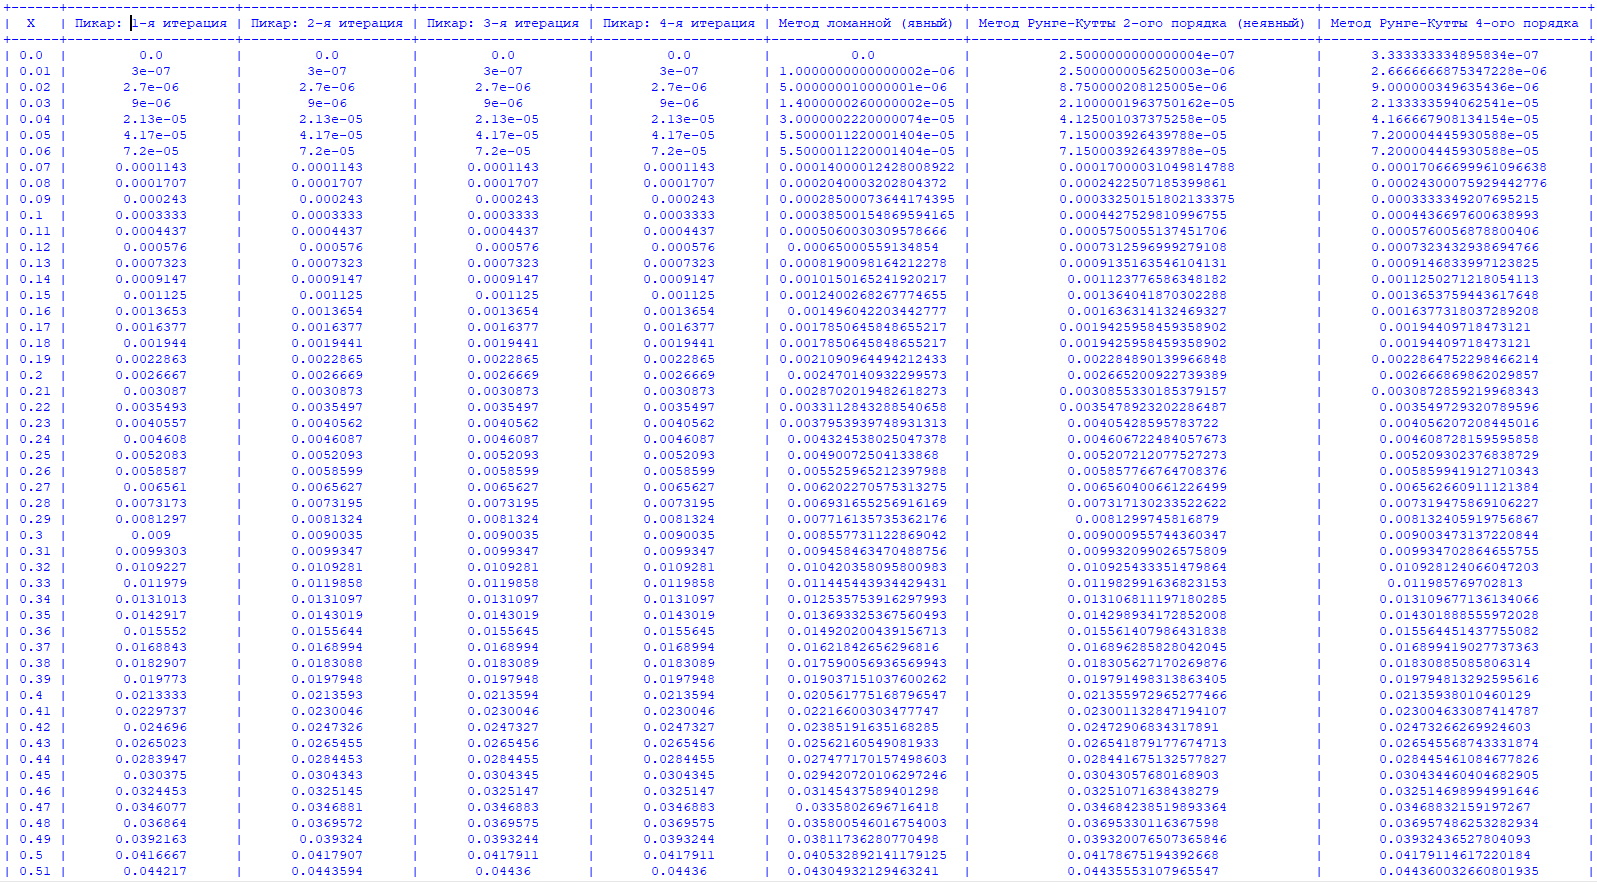
\includegraphics[width=\linewidth]{1}
		\caption{}
		\label{fig:1}
	\end{figure}
	
	\begin{figure}[H]
		\centering
		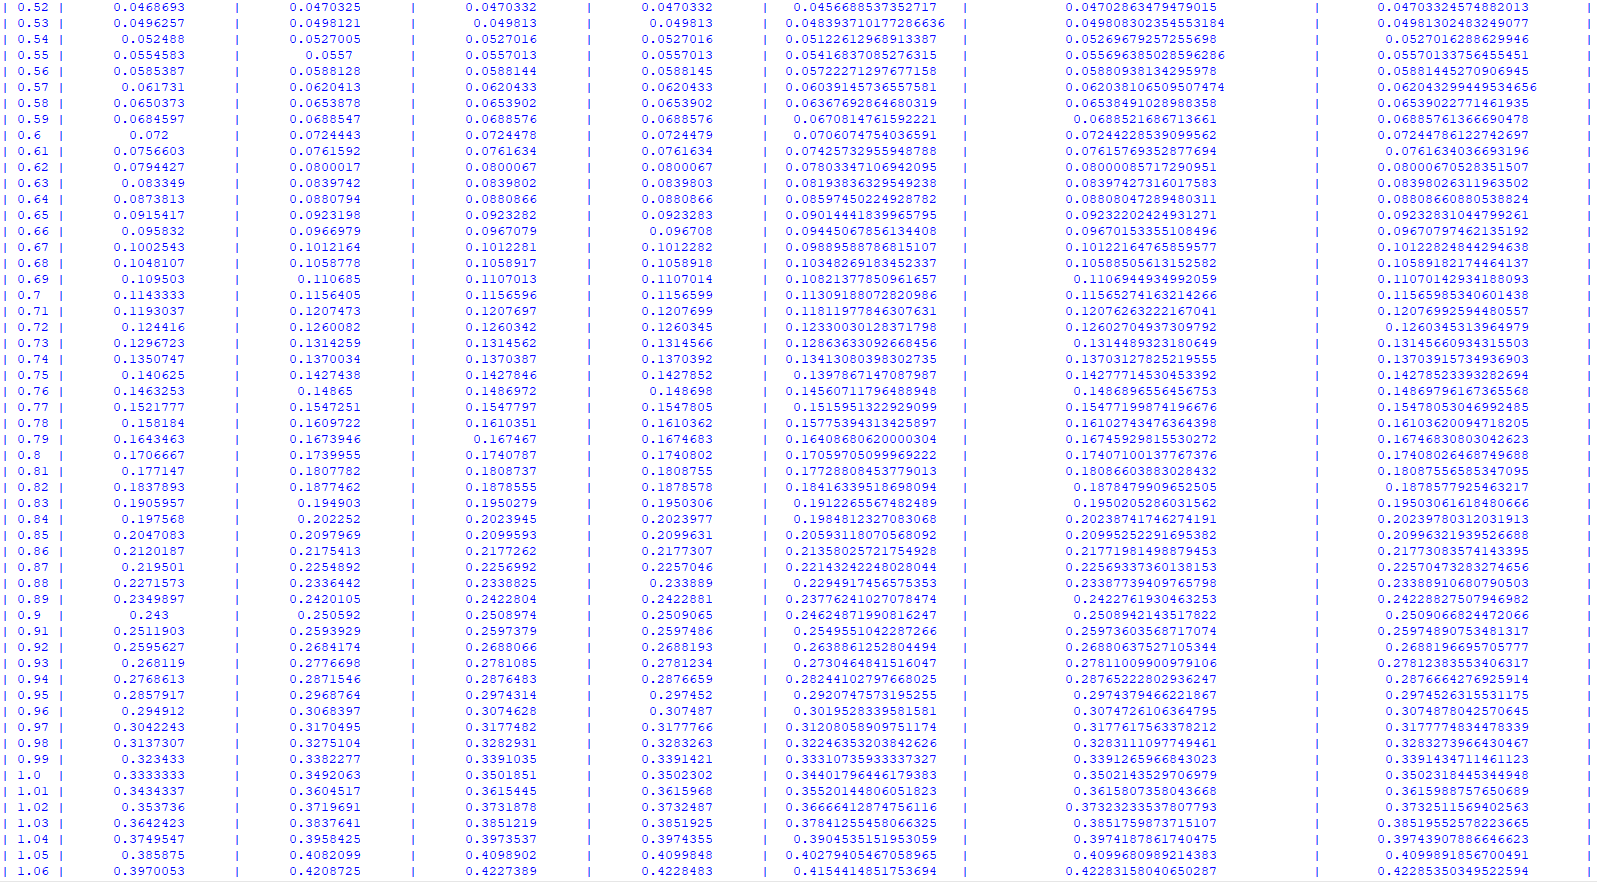
\includegraphics[width=\linewidth]{2}
		\caption{}
		\label{fig:2}
	\end{figure}

	\begin{figure}[H]
		\centering
		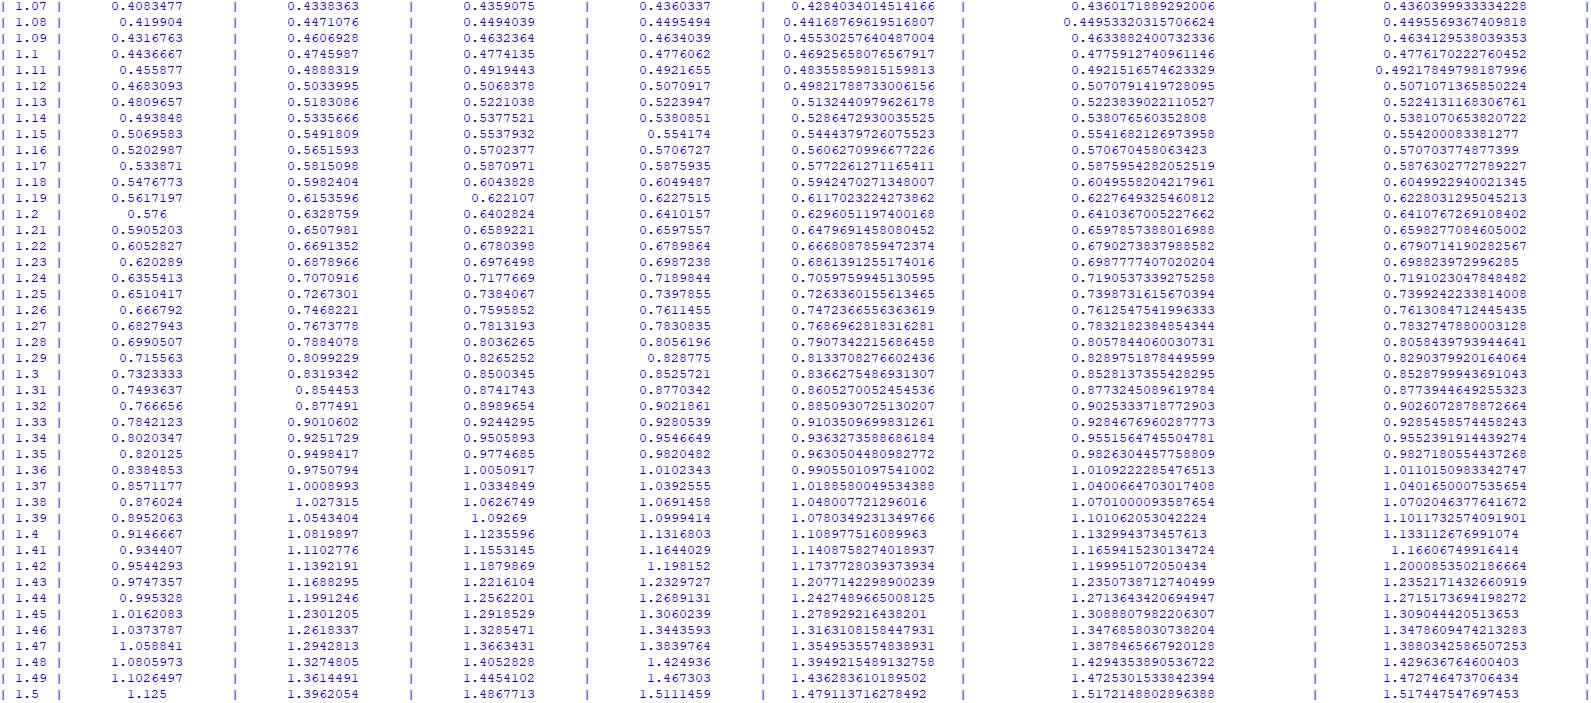
\includegraphics[width=\linewidth]{3}
		\caption{}
		\label{fig:3}
	\end{figure}
	
	\section{Ответы на вопросы}
	\begin{enumerate}
		\item Укажите интервалы значений аргумента, в которых можно считать решением заданного уравнения каждое из первых 4-х  приближений Пикара. Точность результата оценивать до второй цифры после запятой. Объяснить свой ответ.
		\begin{enumerate}
			\item 1ое приближение: [0 - 0.86] Значение функции совпадает c приближением на данном интервале до 2ух знаков. 
			\item 2ое приближение: [0 - 0.18] Значение функции совпадает c приближением на данном интервале до 2ух знаков. 
			\item 3ье приближение: [0 - 1.36] Значение функции совпадает c приближением на данном интервале до 2ух знаков.
			\item 4ое приближение: [0 - 1.51] Значение функции совпадает c приближением на данном интервале до 2ух знаков.
		\end{enumerate}
		\item Пояснить, каким образом можно доказать правильность полученного результата при фиксированном значении аргумента  в численных методах. 
		\begin{enumerate}
			\item Численные методы зависят от шага, по этому мы сравниваем значение полученные Эйлером при разных его величинах. На пример: берем шаг равный 0.00001 получаем (для примера) 200, а при 0.0000001 получаем 300. Видим, что слишком большая разница которая нас не устраивает, продолжаем уменьшать шаг. И так до тех пора пока не получаем устраивающую нас точность. Правда есть вероятно того, что мы выйдем за разрядность и будет происходить округление.
		\end{enumerate}
		\item Из каких соображений выбирался корень уравнения в неявном методе?
		\begin{enumerate}
			\item Выбирается наименьший из двух корней для сохранения непрерывности функции
		\end{enumerate}
		\item Каково значение функции при x=2, т.е. привести значение u(2).
		\begin{figure}
			\centering
			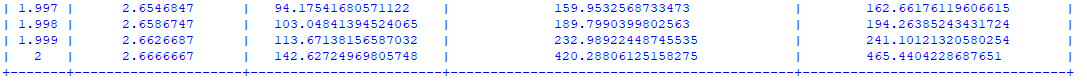
\includegraphics[width=\linewidth]{4}
			\caption{}
			\label{fig:4}
		\end{figure}
		
		\begin{enumerate}
			\item Около 465
		\end{enumerate}
	\end{enumerate}

	\section*{Список литературы}
	\begin{thebibliography}{3}
		\bibitem{Gradov 2020}
			Градов В.М. Курс лекций по Моделированию - 2020
		\bibitem{Kalitkin}
			Калитикин Численнные методы URL https://studfile.net/preview/878067/
		
	\end{thebibliography}
	

\end{document}